\documentclass{article}
\usepackage{graphicx}
\usepackage{amsmath}
\usepackage{hyperref}
\usepackage{pgfplots}
\usetikzlibrary{pgfplots.groupplots}
\pgfplotsset{compat=newest} 
\usepackage{booktabs}
\usepackage{algorithm}
\usepackage{algpseudocode}
\usepackage[left=1in, right=1in, top=1in, bottom=1in]{geometry}

\title{Alignment	algorithms	for	probabilistic	sequences}
\author{Marina Zhou 260898607 , Jessie Xu 260966881, Juliette Xu 260960059}
\date{December 15, 2023}

\begin{document}

\maketitle

\section*{Introduction}
BLAST (Basic Local Alignment Search Tool) - a tool introduced in 1990 by Altschul et al.[1], that is often used to find alignments between short query sequences and a long genome. This is rather useful in many genome analyses. However, BLAST does not work when the genome (database) sequence is probabilistic. Therefore an analog of BLAST that works for probabilistic sequences is necessary. In this report, we present a variation (probabilistic adaptation) of BLAST that can align short (non probabilistic) queries to long probabilistic sequences. A sample of chromosome 22 from the predicted BoreoEutherian ancestor sequence was used to test and evaluate the algorithm. \\
\\
Our proposed algorithm takes two inputs: a probabilistic database sequence and a query sequence. It aims to output a local alignment with the highest score. To test the accuracy of the algorithm, we picked a random starting position in the probabilistic database. 10 random short sequences of 100 nucleotides were generated by selecting nucleotides randomly according to the probabilities at each position. We also implemented additional random substitutions, additional, and deletions of the nucleotides to test the robustness of the method. The accuracy of the algorithm was evaluated by verifying whether the algorithm could accurately output the alignment between the query sequence and the corresponding segment of the database sequence from which the query was derived.\\
\\
There are three main differences between our proposed solution and the traditional BLAST algorithm. First, we proposed a new matching scheme based on the given probabilistic database. Second, the gap penalty (linear) is defined as the average confidence of the database. Third, during the scan for hits stage of the algorithm, this algorithm does not seek a perfect match. Our proposed algorithm will consider any matches above a certain threshold (e.g., $95\%$ between the w-mer from the query and the w-mer from the database). As a result, the algorithm takes into account a wider range of matches, thus improving the accuracy with probabilistic inputs. However, this approach will also significantly increase the running time of the algorithm, making the trade-off between efficiency and accuracy an important factor to consider.\\
\\
Overall, our proposed solution performed very well. When no random swaps, additions, and deletions of nucleotides were used to generate the testing query, it can produce a 100\% accurate alignment. When 5 random swaps, additions, and deletions of nucleotides were used to generate the testing query, the program can find an alignment 30\% of the time with an average search time of 495.49 seconds. The reported alignments were at most 2 positions off from where they were generated. We also discovered that, when compared with the traditional BLAST algorithm, the running time of our algorithm will be negatively affected by large mer size. The algorithm is more efficient when we use a large w-mer.\\
\\


\section*{Methodology}
\subsection*{Input and Output}
The algorithm takes two inputs: the sequence database file and the probabilistic database database file. The database sequence contains a single string, where each character represents a nucleotide. The probabilistic database contains a series of decimal values separated by a space. These decimal numbers represent the probability of the corresponding nucleotide appearing in its position in the database sequence. For instance, if the database sequence begins with the nucleotide 'A', and the probability of 'A' occurring in this position is 0.7, then the first decimal in the probabilistic database will be noted as 0.7. \\
\\
The algorithm outputs 1) the optimal local alignment between the query sequence and the database sequence, 2) the score of the optimal alignment, 3) the running time, and 4) the starting index of the local alignment in the database sequence.\\

\subsection*{Pre-Processing}
\subsubsection*{Convert input}
We began by converting the sequences in the sequence database file into lists. Then, we aggregated the lists into a larger list named $L_1$. Similarly, we converted the probability sequences from the probabilistic database file into lists and aggregated them into $L_2$.

\subsubsection*{Calculate gap penalty}
\label{sec:gap}
We iterate over $L_2$ to compute the average value of each probabilistic nucleotide. We then used this average as our gap penalty. Note that in our current implementation, as the database contains only one sequence, we directly do $sum(L1[0])$. However, in cases where the database contains multiple sequences, we should calculate the average probability across all sequences, as described above.\\

\subsubsection*{Find probability of all nucleotide}
\label{sec:nucprob}

The probabilistic database only contains the probabilities of the corresponding nucleotides appearing in their positions in the database sequence. Therefore, we need to calculate the probabilities of the other three nucleotides occurring at the same positions. First, we create a matrix \( M \) with the four nucleotides (A, T, G, C) as rows and the sequence index as columns. Then, we iterate through \( L2 \) to find the probability of each nucleotide and record it in \( M \). Finally, we subtracted this probability from 1 and divided the result by three to determine the probabilities of the remaining three nucleotides. For example, for a nucleotide "A" at index 1 with a probability of 0.7, we will have "T", "G", and "C" at index 1 with a probability of \( \frac{1-0.7}{3} = 0.1 \) each.\\

\subsection*{New Scoring Scheme}
\label{sec:scoring}
In this algorithm, we introduced a new scoring scheme based on the given probabilistic database. If two nucleotides match, we plus the probability (denoted as a decimal) of the nucleotide at position $i$ in the database sequence. If the two nucleotides mismatch, we minus the probability of the nucleotide at position $i$ in the database sequence. The alignment score is calculated by summing up the score of each nucleotide. Table 1 and Table 2 gave an example grading scheme concerning the nucleotide A at the first position in the database.\\
 %%%%%%%%% Table One %%%%%%%%%%%
\begin{table}[htbp!]
\centering

\begin{tabular}{|l|c|}
\hline
\textbf{Nucleotide k at position 1} & \textbf{Probability} \\ \hline
A & 0.7 \\ 
T & 0.1 \\ 
G & 0.1 \\ 
C & 0.1 \\ \hline
\end{tabular}
\caption{Probability of nucleotides at position 1.}
\label{tab:nucleotide_probability}
\bigskip

%%%%%%%%% Table Two %%%%%%%%%%%

\begin{tabular}{|l|c|c|}
\hline
\textbf{Nucleotide in Dataset} & \textbf{Nucleotide in Query} & \textbf{Score} \\ \hline
A & A & +0.7 \\ 
A & T, G, C & -0.7 \\ \hline
\end{tabular}
\caption{Score of matches and mismatches regarding Nucleotide A at position 1.}
\label{tab:score_A}
\bigskip

%%%%%%%%% Table Three %%%%%%%%%%%

\begin{tabular}{|l|c|c|}
\hline
\textbf{Nucleotide in Dataset} & \textbf{Nucleotide in Query} & \textbf{Score} \\ \hline
T & T & +0.1 \\ 
T & A, G, C & -0.1 \\ \hline
\end{tabular}
\caption{Score of matches and mismatches regarding Nucleotide T at position 1.}
\label{tab:score_T}
\end{table}

\subsection*{Probabilistic BLAST}
\subsubsection*{Creating w-mers}
This step is the same as the traditional BLAST algorithm. We started with a given substring size \( w \), pre-processed lists \( L_1 \) containing sequences from the database, and the input query. We extracted all w-mers and their starting index from the database and the input query. These w-mers were then stored in two separate dictionaries: \( D_1 \) for the database and \( D_2 \) for the query. In these dictionaries, each w-mer serves as a key, and its value is the list of indices where this w-mer appears in the sequence. For example, a dictionary \{ \text{"ATG"}: [1, 10] \} indicates that the substring "ATG" appears at both the first and tenth indices of the sequence.\\
\subsubsection*{Finding Hit}
For finding hits, we use a probabilistic approach instead of simply identifying identical pairs of w-mers and database words. We iterate over each w-mer in \(D_1\) and compare it to every database word in \(D_2\). If the pair has a similarity score more or equal to $95\%$, we shall use them for doing sequence extensions. This similarity score is calculated by comparing the alignment score of a w-mer and a database word, using the \hyperref[sec:scoring]{new scoring scheme}. If the similarity score is greater than or equal to \(0.95 \times w\), where \(w\) represents the size of the w-mer, We take the current w-mer as the key, and a list of tuples (matched-index, similarity score) that sorted from highest similarity score to lowest similarity score as value and add the key-value pairs to a new dictionary \(D_3\).
Here is an example of $D_3$ with $w=4$: \{"ATCG": [(5, 4.0), (8, 3.8)]\}. It represents that the w-mer "ATGC", has a hit with the database word starting at index 5 with a similarity score of 5, and also has a hit with the database word starting at index 8 with a similarity score of 3.8. \\

\subsubsection*{Ungapped Extension}
We loop through each alignment in $D_3$. These initial alignments are termed 'seeds'. We first extend the sequence to the right. As we add each nucleotide, we record the current similarity score and position of the newly added nucleotide. We keep going right until the similarity score of the current alignment becomes smaller than that of the seed. Among the set of nucleotides available for extension, we extend our sequence to the one with the highest similarity score. The same procedure is applied to the left side but in a reverse direction. As the plot illustrates, we start or extend from a seed that has a similarity score of 2.7. We gradually reach a similarity score of 4.3 at the 5th nucleotide, then drop to a similarity score of 2.5 at the 11th nucleotide. At this point, we must stop the extension because $2.5<2.7$. In the range from no extension to extending 11 nucleotides, we select the highest similarity score of 4.3, therefore extending our sequence by 5 nucleotides.\\

\begin{figure}[htbp]
\centering
\begin{tikzpicture}
\begin{axis}[
   width=0.8\textwidth, 
    height=0.4\textheight, 
    title={Ungapped Extension Phase},
    xlabel={number of nucleotides extend to},
    ylabel={Similarity},
    xmin=0, xmax=12, ymax=4.5,
    xtick={0,1,2,3,4,5,6,7,8,9,10,11,12},
    ytick={0, 1, 2, 2.1, 2.2, 2.3, 2.4, 2.5, 2.6, 2.7, 2.8, 2.9, 3.0, 3.1, 3.2, 3.3, 3.4, 3.5, 3.6, 3.7, 3.8, 3.9, 4.0, 4.1, 4.2, 4.3, 4.4, 4.5},
    legend pos=north west,
    ymajorgrids=true,
    grid style=dashed,
]

\addplot[
    color=blue,
    mark=triangle*,
    ]
    coordinates {
    (0,2.7)(1,2.8)(2,3)(3,3.3)(4,3.5)(5,4.3)(6,4.0)(7,3.6)(8,3.3)(9,3.2)(10,2.8)(11,2.5)
    };
\legend{Similarity}
\draw[dashed, thick] (axis cs:0,2.7) -- (axis cs:12,2.7);
\node[align=center, text width=3cm] at (axis cs:4,2.78) {Similarity of Seed};

\draw[dashed, thick] (axis cs:0,2.5) -- (axis cs:12,2.5);
\node[align=center, text width=8cm] at (axis cs:8,2.55) {$2.5 < 2.7$, end extension at the 11th nucleotide};

\draw[dashed, thick] (axis cs:0,4.3) -- (axis cs:12,4.3);
\node[align=center, text width=8cm] at (axis cs:8.8,4.13) {4.3 is the maximum similarity, extend sequence to the 5th nucleotode};

\end{axis}
\end{tikzpicture}
\caption{Plot of the Right Ungapped Extension Phase.}
\label{fig:ungappedextension}
\end{figure}


\subsubsection*{Calculating E-Value}
After we get the ungapped extended alignments, we calculate the e-value of each alignment to ensure the alignments are not given by chance. We first set a threshold for the e-value, and use the formula to calculate the the e-value of the current alignment. If the e-value exceeds this threshold, we discard the alignment. For alignments with a small e-value, we proceed with the gapped extension.

\subsubsection*{Gapped Extension}
For the gapped extension, we use an alternative Needleman-Wunsch algorithm. This algorithm takes two aligned sequences --- one from the query and the other from the sequence database, along with a probabilistic matrix and a \hyperref[sec:gap]{gap penalty}. The algorithm begins by initializing a score matrix and a backtrack matrix. The score matrix is used as the scoring matrix in the traditional Needleman-Wunsch algorithm, but it stores the \hyperref[sec:nucprob]{score of similarity} of the current alignment. The backtrack matrix records the decisions we made (match, mismatch, gap in seq1, or gap in seq2). We start filling our two matrices following the \hyperref[sec:scoring]{new scoring scheme} like what we do in the traditional Needleman-Wunsch algorithm, and then backtrack to get the optimal alignment. \\

\section*{Results}
\subsection*{Overview}
To evaluate our algorithm, we used a section of chromosome 22 from the predicted BoreoEutherian ancestor sequence as the probabilistic database. The input sequences we used were generated by selecting an index in the chromosome 22 sequence randomly and then creating a query of n nucleotides. To determine the nucleotide at a given position in the query, we used the probability of each nucleotide at the position in the database. As such, the likelihood of a nucleotide being chosen for the query sequence was directly proportional to the probability of that nucleotide being the true nucleotide at that position. Random substitutions, insertions, and deletions were performed on the query sequence at various specified rates. \\
\\
To test our algorithm, 11 query datasets were generated with different combinations of nucleotide substitution, insertions/deletions at rates (insert/delete 5,10 nucleotides). The datasets are generated from independently sampled queries of length 100. The results’ accuracy focuses on the starting index s of the database query which the random sequence was generated based on, and compares the difference to the starting index of the database query alignment calculated by the algorithm. This measures the accuracy, as the “optimal” alignment in theory would be the sequence in the database which starts at index s since that was used to generate the random sequence used as input. Thus the difference in starting index could suggest how “off” (inaccurate) the alignment/match found is to the actual alignment.\\

\subsection*{no swaps, add, and deletion}
The initial dataset we ran the algorithm against was the default setting where we only used the random sequences we generated, with no swaps, additions, or deletions. The matching threshold used requires there to be at least a $95\%$ match for the ungapped phase and the w-mer size is 11 (unless otherwise specified, these conditions were used for evaluation). For this input dataset, we were able to get an alignment for 8 out of the 10 input queries. For the queries that we were able to find an alignment, the accuracy was promising as we were able to align with the exact starting indexs that were used to generate the random queries. The average score for this was 77.7563 and the standard deviation for the scores was 4.1879.\\

\subsection*{5 swaps}
Next, we tested our algorithm with different variating combos of substitutions, addition, and deletion. Initially, we only added 5 random swaps in our input queries and the algorithm was pretty successful at finding alignments. It was able to find an alignment for 10 out of the 10 input queries used. As for alignment accuracy, similar to the previous dataset, it was also able to find exact matches for all the alignments. The average score was 80.52533 and the standard deviation for the scores was 5.15049.\\

\subsection*{5 swaps, 5 add, and 5 deletions}
Then we tried to find alignments with 5 substitutions, 5 additions and 5 deletions. For our e-value, we used 0.001 and we had the threshold for word matching in the ungapped phase to be $95\%$, similar to before. With this, our algorithm struggled to find alignments, as only 1 out of the 10 input queries was able to produce an alignment. The accuracy of the alignment was decent, as it was able to find a starting index very close to the actual starting index. The calculated starting index was 77807, compared to the actual starting index which was 77810, which is only 3 nucleotides difference in index.



\subsection*{relax constraints in 3 for e-value and exact matching threshold}
In an attempt to improve the results of the alignment with this combination of substitution, additions, and deletions, we tried to relax the constraints (i.e. e-value, and matching threshold). For the modifications to the constraints, we increased the e-value from 0.001 to 10 and lowered the matching threshold to $90\%$ instead of the previous $95\%$. However, the results we got did not present significant improvement, but rather a lower accuracy in comparison. Again, only one input query was able to produce an alignment output. Even though the region was still fairly close to the actual region, the difference in position for the starting index is 8 (actual = 4388, calculated = 4396), which is a lower accuracy.\\

\subsection*{addition and deletion}
We focused on either only adding or deleting nucleotides from the sequence next, without any substitutions, and using the same constraints as before. The addition/deletion was performed on 4 independent datasets, 2 being the addition/deletion of 5 nucleotides and 2 being the addition/deletion of 10 nucleotides. The results for addition/deletion had a similar pattern based on the number of nucleotides changed. The algorithm was able to find more alignments when there were only 5 nucleotide modifications, with gaps in both query and database sequences.

\begin{table}
    \centering
    \begin{tabular}{cccccc}
         & number of matches & average score & score standard deviation & average accuracy & accuracy standard deviation\\
         &  &  &  &  & \\
         &  &  &  &  & \\
         &  &  &  &  & \\
         &  &  &  &  & \\
         &  &  &  &  & \\
    \end{tabular}
    \caption{setting}
    \label{tab:my_label}
\end{table}


\section*{Discussion and future	work}
\subsection*{Discussion}
The algorithm we implemented was able to successfully perform the alignment of a short (non probabilistic) query to a long probabilistic sequence. Matches were decent, and here are some statistics of our matchings\\
\\
One advantage of our implementation is that w-mer size does not affect the matching results. This is because, for the determinization of the w-mers, the threshold is for there to be a 95$\%$ match from the w-mer to the database sequence, as opposed to requiring a strict perfect match. However, using a larger w-size will increase the efficiency of our algorithm since the maximum possible number of hits to do the gapped extension will be less. For example, if the database sequence is of length 100 nucleotides. If the w-mer size is 99, then there will only be a maximum of 2 hits which can then be used to do gapped extension. Comparing this to a w-mer size of 10, the maximum number of hits is significantly higher, which then increases the overall running as the gapped extension phase needs to be performed for every single hit.\\
\\
As with any algorithm, there are also limitations to the presented algorithm. In the case of the algorithm, the given databases are probabilistic. Thus for the expansion step, we are expanding all possible w-mers, instead of only the top k possible w-mers. This then presents a trade-off between efficiency and accuracy. In our case, we chose accuracy. 

\subsection*{Future Work}
In our algorithm, we used a basic (brute force) method to produce all the w-mers. The method is such that we use a for loop to iterate through the whole input sequence, indexing the [i: i+w] slice of the input sequence at each iteration. However, there are known optimizations that can be implemented. An example of such is to use the Biopython library which is an open-source Python library specifically designed to enable bioinformatics and computational biology tasks. By using the Seq class in the Biopython library, we can efficiently parse through the input sequence and return all the w-mers found. The implementation of such will be able to further improve our algorithm’s efficiency.\\
\\
Another optimization that we can do for our algorithm, is in the gapped extension phase. Currently, the algorithm uses the Needleman Wunsch (NW) algorithm for the gapped extension phase, however, a modified version of NW could increase the efficiency of the algorithm. The idea of the modification is suggested by Altschul et al.[2] where the alignments produced are confined to a predefined strip of the dynamic programming path graph by heuristic methods. Then the algorithm “considers only alignments that drop in score no more than Xg below the best score yet seen. The algorithm is able thereby to adapt the region of the path graph it explores to the data.” (Altschul et al.[2]) \\

\section*{Bibliography}




\end{document}
